\documentclass[a4paper,12pt]{toptesi}
\usepackage[ansinew]{inputenc}
%\usepackage[utf8]{inputenc}
%\usepackage[latin1]{inputenc}
\usepackage[italian]{babel}
\usepackage{amsmath}
\usepackage{amssymb}
\usepackage{amsfonts}
%\usepackage{multirow}
\usepackage{graphicx}
\usepackage{url}
\usepackage{listings, xcolor}
\lstset{
tabsize = 4, %% set tab space width
showstringspaces = false, %% prevent space marking in strings, string is defined as the text that is generally printed directly to the console
numbers = left, %% display line numbers on the left
commentstyle = \color{green}, %% set comment color
keywordstyle = \color{blue}, %% set keyword color
stringstyle = \color{red}, %% set string color
rulecolor = \color{black}, %% set frame color to avoid being affected by text color
basicstyle = \small \ttfamily , %% set listing font and size
breaklines = true, %% enable line breaking
numberstyle = \tiny,
}

\begin{document}

\NomeMonografia{}
\monografia{Prova Finale \\ Gestione Magazzino Lego}
\ateneo{Politecnico di Torino}
\logosede{logo/LogoPoliTo.eps}
\corsodilaurea{Ingegneria Gestionale Classe L8}
%\relatore{prof.\ Fulvio Corno}
\sedutadilaurea{Dicembre 2020}
\candidato{Relatore prof. Fulvio Corno \\ Candidato Salvatore Dipace}

\frontespizio

\tableofcontents

\chapter*{Proposta progetto}
\addcontentsline{toc}{chapter}{Proposta Progetto}


Di seguito si riporta la proposta integrale del progetto con alcune modifiche introdotte durante lo svolgimento del lavoro

\section{Studente proponente}
s232047 - Salvatore Dipace

\section{Titolo della proposta}
Collezionisti LEGO - analisi del magazzino dei pezzi

\section{Descrizione del problema proposto}
Considerato un magazzino di pezzi LEGO ampliato negli anni attraverso l'acquisto di set o di mattoncini sfusi, si vuole sviluppare un'applicazione che permetta di analizzare le potenzialit� dello stesso in termini di numero massimo di set (ufficiali o mock proposti da appassionati) costruibili contemporaneamente con i pezzi a disposizione.
L'applicazione permette inoltre di capire quali sono i set che conviene acquistare per colmare il gap tra il magazzino a disposizione e un insieme di set a cui si � interessati per minimizzare le spese e ottimizzare l'utilizzo delle risorse a disposizione.

\section{Descrizione della rilevanza gestionale del problema}
Si tratta di un problema di gestione di risorse a disposizione per ottimizzare una funzione obiettivo.
L'interesse verso questo gioco � rimasto immutato negli anni e coinvolge non solo bambini, ma anche adulti collezionisti. Per alcune persone si tratta anche una forma di investimento che si rivaluta negli anni dopo che un set viene messo fuori produzione.
Potrebbe quindi essere interessante fornire uno strumento che permetta di capire come ottimizzare il magazzino a disposizione.

\section{Descrizione dei data-set per la valutazione}
Il data-set � reperibile qui: \url{https://rebrickable.com/downloads/}
Inizialmente si � lavorato con quello pubblicato su \\ \url{https://www.kaggle.com/rtatman/lego-database/}, ma il primo mette a disposizione dati aggiornati quotidianamente su una base dati strutturata nello stesso modo.
Per ogni set commercializzato (tabella \texttt{sets}) sono elencati tutti i pezzi necessari (tabella \texttt{inventory\_parts}). Serve aggiungere una tabella nuova per gestire il magazzino dei pezzi sfusi a disposizione del collezionista.



\chapter*{Problema affrontato}
\addcontentsline{toc}{chapter}{Problema affrontato}
L'applicazione proposta � un semplice prototipo di strumento che i collezionisti del gioco LEGO potrebbero utilizzare per poter valutare le potenzialit� dei pezzi a disposizione in un ipotetico magazzino. I problemi affrontati sono due:
\begin{enumerate}
	\item quali set si possono costruire (interamente o parzialmente) con i pezzi a disposizione;
  \item stabilito un obiettivo espresso attraverso un insieme di set che si vorrebbe costruire, capire 
\begin{itemize}
	\item quali e quanti pezzi mancano in magazzino;
	\item quali set conviene acquistare per colmare il gap.
\end{itemize}
\end{enumerate}

Per il primo problema l'utente pu� scegliere una o pi� serie di interesse. Scelta una percentuale di completamento del set, si mostrano a video le combinazioni possibili con il numero pi� alto di set.
Pi� la percentuale si abbassa, pi� alta sar� l'insieme dei set costruibili.
Si utilizza l'algoritmo della ricorsione in quanto si tratta di un caso di studio simile al problema dello zaino.

Il secondo problema � affrontato per passi successivi:
\begin{itemize}
	\item scelta delle serie da analizzare
	\item creazione di un grafo pesato non orientato con le seguenti caratteristiche:
\begin{itemize}
	\item i nodi sono costituiti dai set
	\item esiste un arco tra due nodi solo se il coefficiente di accoppiamento tra i due set 
	rappresentati dai nodi � superiore a una soglia scelta da interfaccia. Il coefficiente corrisponder� al peso dell'arco. 
\end{itemize}
	Il coefficiente di accoppiamento x tra il nodo A e quello B � definito come
\begin{equation*}
\text{x}= \frac{\left(\text{numero pezzi in comune}\right)^{2}}{\left( \text{numero pezzi set A} \right) \left( \text{numero pezzi set B} \right)}
\end{equation*}

	\item si sceglie un set tra quelli del grafo e si mostra l'albero di visita
	\item si calcola la lista di pezzi mancanti in magazzino per poter costruire i set che compongono l'albero di visita
	\item si calcola l'insieme pi� piccolo di set che conviene acquistare per colmare il gap in base a una percentuale di completamento scelta da interfaccia. Questo perch� l'utente potrebbe decidere di coprire parte del gap acquistando pezzi sfusi secondo considerazioni economiche.
\end{itemize}

L'interfaccia, senz'altro migliorabile, cerca di guidare le scelte dell'utente attivando i bottoni delle varie funzionalit� solo quando si sono completati i passi precedenti.


\chapter*{Descrizione del data-set utilizzato per l'analisi}
\addcontentsline{toc}{chapter}{Descrizione del data-set}

Il data-set considerato � pubblicato su \url{https://rebrickable.com/downloads/}. La tabelle sono state create con il tool HeidiSQL a partire dal diagramma relazionale a disposizione. I dati, aggiornati ogni giorno, si possono caricare a partire dai file csv di ogni tabella con la funzionalit� di import a partire da file csv.

Non tutte le tabelle della base dati sono servite per le funzionalit� implementate: quelle utilizzate sono schematizzate nella figura \ref{FIG:base_dati}. In grigio � evidenziata una tabella non presente nella base dati pubblicata e introdotta per modellare il magazzino del collezionista.
Il pezzo � univocamente identificato attraverso un codice, il colore e il materiale. Ogni set � composto da uno o pi� pezzi e appartiene a una serie.
Una breve descrizione di ciascuna tabella � indicata nella tabella \ref{TAB:descrizione_base_dati}

\newpage
\vspace{0.5cm} 
\begin{figure}[htbp]
\centering
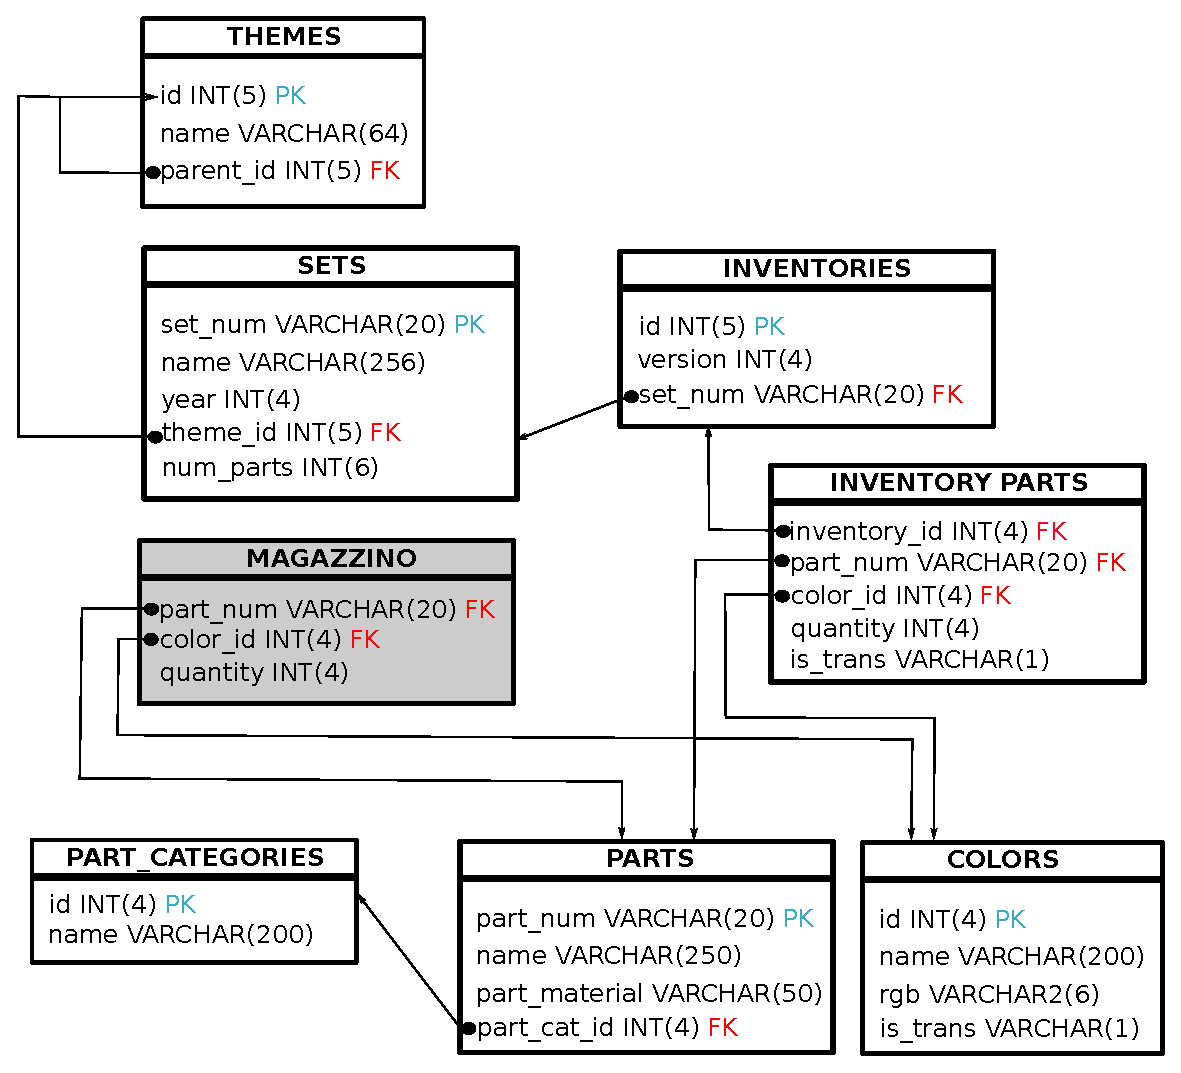
\includegraphics[scale=0.65]{data_set/base_dati.eps}
\vspace{6.5cm} \caption{Base dati considerata dall'applicazione di gestione/analisi magazzino Lego}
\label{FIG:base_dati}
\end{figure}
\vspace{0.5cm} 

\newpage


\begin{table}[htbp]
\begin{center}
\begin{tabular}{||p{0.23\linewidth}|p{0.18\linewidth}|p{0.1\linewidth}|p{0.15\linewidth}|p{0.25\linewidth}||}
\hline
{\bfseries tabella} & scopo & numero record & chiave primaria PK & chiavi esterne FK\\
\hline
\hline
\texttt{themes} & elenco di tutte le serie in commercio & circa 500 & campo id & il campo parent\_id assume solo valori contenuti nel campo id. Se valorizzato, indica che la serie un filone di un'altra principale \\
\hline
\texttt{sets} & elenco di tutti i set in commercio & circa 15000 & campo \texttt{set\_num} & il campo \texttt{theme\_id} assume solo valori contenuti nel campo id della tabella theme. Ogni set � quindi associato a una serie. \\
\hline
\texttt{parts} & elenco di tutti i pezzi in commercio & circa 35000 & campo \texttt{part\_num} & \\
\hline
\texttt{colors} & elenco di tutti i colori dei pezzi & circa 200 & campo \texttt{id} & \\
\hline
\texttt{inventories} e \texttt{inventory\_parts} & relazionano i set e i pezzi che lo compongono & circa 750000 & & campi \texttt{part\_num}, \texttt{color\_id} e \texttt{inventory\_id}\\
\hline
\texttt{colors} & elenco di tutti i colori dei pezzi & circa 200 & id & \\
\hline
\texttt{magazzino} & contiene i pezzi a disposizione del collezionista. In continuo aggiornamento & & & campi \texttt{part\_num} e \texttt{color\_id}\\

\hline
\hline
\end{tabular}
\caption {\label{TAB:descrizione_base_dati}  Descrizione e caratteristiche delle tabelle utilizzate}
\end{center}
\end{table}
\vspace{0.5cm}


\chapter*{Descrizione delle strutture dati e degli algoritmi utilizzati}
\addcontentsline{toc}{chapter}{Descrizione delle strutture dati e degli algoritmi}
L'applicazione � stata sviluppata seguendo il pattern MVC. Di seguito si descriveranno le strutture dati utilizzate e gli algoritmi implementati.

\section{Organizzazione delle classi}

Il package \texttt{model} contiene la classe Model che espone i metodi per il Controller. Per una pi� semplice leggibilit� e manutenzione del codice, si sono creati pi� package interni:
\begin{itemize}
\item \texttt{bean}: ospita tutte le classi che modellano gli oggetti;
\item \texttt{exception}: raccoglie le eccezioni. Si  � lavorato con una sola eccezione generica, ma se ne potrebbero creare diverse per ogni situazione specifica.  
\item \texttt{ricorsione}: qui si trovano le classi che si occupano di risolvere i problemi con l'algortimo della ricorsione. Sono due perch� l'algoritmo di ricorsione seguito per il problema di come colmare il gap del magazzino � leggermente diversa. Si � sviluppata anche una classe di test
\item \texttt{graph}: contiene la classe che  espone i metodi per creare il grafo e le relative visite. E' accompagnata da una classe di test
\end{itemize}
Infine c'� il package \texttt{db} con la classe DAO e quelle di test e utility.

\section{Ricorsione}

L'algoritmo di ricorsione � stato utilizzato per trovare le sequenze pi� lunghe di set costruibili con il magazzino a disposizione e per determinare l'insieme pi� piccolo di set da acquistare per colmare il gap del magazzino, per raggiungere un determinato obiettivo.

\subsection{Ricorsione per l'analisi delle potenzialit� del magazzino}

La soluzione parziale � rappresentata da una lista di Set. E' una soluzione valida del problema se non sono state trovate fino a quel momento liste di Set con dimensione maggiore o equivalenti.  Due liste di set sono equivalenti se hanno stessa dimensione e contengono gli stessi set anche in ordine diverso. Ci possono essere pi� soluzioni valide: quindi la struttura dati considerata sar� una lista di liste di Set.
Il codice dell'algoritmo implementato � il seguente

\begin{lstlisting}[language = Java , frame = trBL  , escapeinside={(*@}{@*)}]
	protected void scegli(List<Set> parziale, List<List<Set>> best, int percentualeCompletamento) {

		if (!parziale.isEmpty() && parziale
				.size() >= ((best == null || best.isEmpty() || best.get(0) == null) ? 0 : best.get(0).size())) {
			// trovato soluzione migliore

			if (parziale.size() > ((best == null || best.isEmpty() || best.get(0) == null) ? 0 : best.get(0).size())) {
				best.clear();
			}

			if (!areSoluzioniEquivalenti(parziale, best)) {
				java.util.List<Set> temp = new ArrayList<Set>();
				temp.addAll(parziale);
				best.add(temp);
			}

		}

		for (Set s : getSets()) {
			if (!parziale.contains(s)) {
				// il set non c'� ancora in parziale e provo ad aggiungerlo
				if (areThePartsToBuildTheSetWithTheRequiredPercentageInStock(s, percentualeCompletamento)) {
					//nuova soluzione parziale
					parziale.add(s);
					updateMagazzino(s, "ADD");
					// si delega la ricerca al livello successivo
					scegli(parziale, best, percentualeCompletamento);
					//backtracking
					parziale.remove(s);
					updateMagazzino(s, "REMOVE");
				}

			}

		}

	}

\end{lstlisting}

Quando si considera una nuova soluzione parziale si deve aggiornare il magazzino rimuovendo i pezzi che costituiscono il set scelto. In fase di backtracking si devono invece rimettere in magazzino i pezzi del set rimosso dalla soluzione parziale.

\begin{lstlisting}[language = Java , frame = trBL  , escapeinside={(*@}{@*)}]
protected void updateMagazzino(Set s, String operation) {
		Map<String,Part> parts = s.getParts();

		for (String keyPart : parts.keySet()) {
			if (getMagazzino().containsKey(keyPart)) {
				Part magazzinoPart = getMagazzino().get(keyPart);
				if ("ADD".equals(operation)) {
					magazzinoPart.decrementQuantity(parts.get(keyPart).getQuantity());
				} else {
					magazzinoPart.incrementQuantity(parts.get(keyPart).getQuantity());
				}

			}

		}
	}
\end{lstlisting}

La struttura dati utilizzata per rappresentare il magazzino � una mappa dove la chiave � l'identificativo del pezzo e il valore � l'oggetto pezzo. Per capire se una soluzione parziale � equivalente con una delle soluzioni in quel momento salvate come soluzioni definitive, si usa il metodo

\begin{lstlisting}[language = Java , frame = trBL  , escapeinside={(*@}{@*)}]
	protected boolean areSoluzioniEquivalenti(List<Set> parziale, List<List<Set>> best) {
		if (parziale == null || parziale.isEmpty()) {
			if (best == null || best.isEmpty()) {
				return true;
			} else {
				return false;
			}
		}

		if (best == null || best.isEmpty()) {
			if (parziale == null || parziale.isEmpty()) {
				return true;
			} else {
				return false;
			}
		}

		if (best.get(0).size() != parziale.size()) {
			return false;
		}

		for (List<Set> soluzione : best) {
			/*
			 * //to avoid messing the order of the lists we will use a copy
			 */
			List<Set> soluzioneTemp = new ArrayList<Set>(soluzione);
			List<Set> parzialeTemp = new ArrayList<Set>(parziale);

			Collections.sort(soluzioneTemp);
			Collections.sort(parzialeTemp);

			if (parzialeTemp.equals(soluzioneTemp)) {
				return true;
			}

		}

		return false;
	}
\end{lstlisting}

\newpage

Un set pu� essere aggiunto nella soluzione parziale solo se in magazzino ci sono i pezzi necessari per costruirlo completamente o in parte in base alla percentuale scelta dall'utente. Il metodo implementato � il seguente
\begin{lstlisting}[language = Java , frame = trBL  , escapeinside={(*@}{@*)}]
	protected boolean areThePartsToBuildTheSetWithTheRequiredPercentageInStock(Set s, int requiredPercentage) {
		Map<String, Part> parts = s.getParts();
		Map<String, Part> magazzinoTemp = new HashMap<String, Part>();
		magazzinoTemp.putAll(getMagazzino());

		int availablePartsNumber = 0;
		for (String keyPart : parts.keySet()) {

			if (magazzinoTemp.containsKey(keyPart)) {
				Part magazzinoPart = magazzinoTemp.get(keyPart);

				if (magazzinoPart.getQuantity() < parts.get(keyPart).getQuantity()) {
					availablePartsNumber += magazzinoPart.getQuantity();

				} else {
					availablePartsNumber += parts.get(keyPart).getQuantity();
				}

			}

		}
		int percentage = (availablePartsNumber * 100) / s.getPartsNumber();
		return percentage >= requiredPercentage;

	}
\end{lstlisting}
I metodi sono protetti e non privati per poter essere testati nella classe di test.

\subsection{Ricorsione per l'analisi del gap}
La logica � molto simile alla soluzione precedente. Non si riporta il codice, ma si elencano solo le differenze:
\begin{itemize}
\item la nuova soluzione parziale si genera rimuovendo un set e non aggiungendolo perch� l'obiettivo � trovare l'insieme di set pi� piccolo che colma il gap con la percentuale scelta
\item la nuova soluzione parziale � tale se permette di colmare la parte di gap impostata dall'utente. Se non lo �, il set non viene preso in considerazione e se ne rimuovo un altro
\item in questo caso non deve essere aggiornato il magazzino perch� questo � virtualmente costituito dalla soluzione parziale che si sta considerando in quel momento e che varia a seconda dei sei aggiunti e tolti.
\end{itemize}




\section{Grafo}
Per analizzare gli accoppiamenti tra un insieme di set avendo evidenza di quelli con pi� pezzi in comune, si � costruito un grafo non orientato e pesato. L'arco tra due set esiste se l'accoppiamento tra loro � maggiore di una soglia scelta dall'utente. Per costruire il grafo si � sviluppato il metodo

\begin{lstlisting}[language = Java , frame = trBL  , escapeinside={(*@}{@*)}]
	public Graph<Set, DefaultEdge> creaGrafo(List<Theme> themes, double threshold) throws LegoException {

		Graph<Set, DefaultEdge> graph;

		List<Set> sets = init(themes);

		graph = new SimpleWeightedGraph<Set, DefaultEdge>(DefaultEdge.class);
		Graphs.addAllVertices(graph, sets);

		// aggiungo un arco tra tutti i set, con peso x = coefficiente di accoppiamento
		for (Set s1 : graph.vertexSet()) {
			for (Set s2 : graph.vertexSet()) {
				if (!s1.equals(s2)) {
					Float accoppiamento = calcolaAccoppiamento(s1, s2);
					if (accoppiamento * 100 >= threshold) {
						Graphs.addEdgeWithVertices(graph, s1, s2, accoppiamento);
					}
				}
			}
		}

		return graph;

	}
\end{lstlisting}
mentre il calcolo del coefficiente di accoppiamento tra due set avviene con il metodo

\begin{lstlisting}[language = Java , frame = trBL  , escapeinside={(*@}{@*)}]
	private Float calcolaAccoppiamento(Set s1, Set s2) {

		float coefficienteAccoppiamento;
		// se uno dei due set non ha pezzi -->0
		if (s1.getParts().isEmpty() || s1.getParts().isEmpty()) {
			coefficienteAccoppiamento = 0;

		} else {
			int numeroPezziInComune = 0;
			if (s1.getPartsNumber() >= s2.getPartsNumber()) {
				for (String keyPart : s2.getParts().keySet()) {
					if (s1.getParts().containsKey(keyPart)) {
						if (s1.getParts().get(keyPart).getQuantity() >= s2.getParts().get(keyPart).getQuantity()) {
							numeroPezziInComune += s2.getParts().get(keyPart).getQuantity();
						} else {
							numeroPezziInComune += s1.getParts().get(keyPart).getQuantity();
						}
					}
				}

			} else {
				for (String keyPart : s1.getParts().keySet()) {
					if (s2.getParts().containsKey(keyPart)) {
						if (s2.getParts().get(keyPart).getQuantity() >= s1.getParts().get(keyPart).getQuantity()) {
							numeroPezziInComune += s1.getParts().get(keyPart).getQuantity();
						} else {
							numeroPezziInComune += s2.getParts().get(keyPart).getQuantity();
						}
					}
				}

			}
			coefficienteAccoppiamento = (float) (numeroPezziInComune * numeroPezziInComune)
					/ ((s1.getPartsNumber() * s2.getPartsNumber()));
		}

		return coefficienteAccoppiamento;
	}
\end{lstlisting}

 	

\chapter*{Diagramma delle classi delle parti principali}
\addcontentsline{toc}{chapter}{Diagramma delle classi}
\begin{figure}[htbp]
\centering
    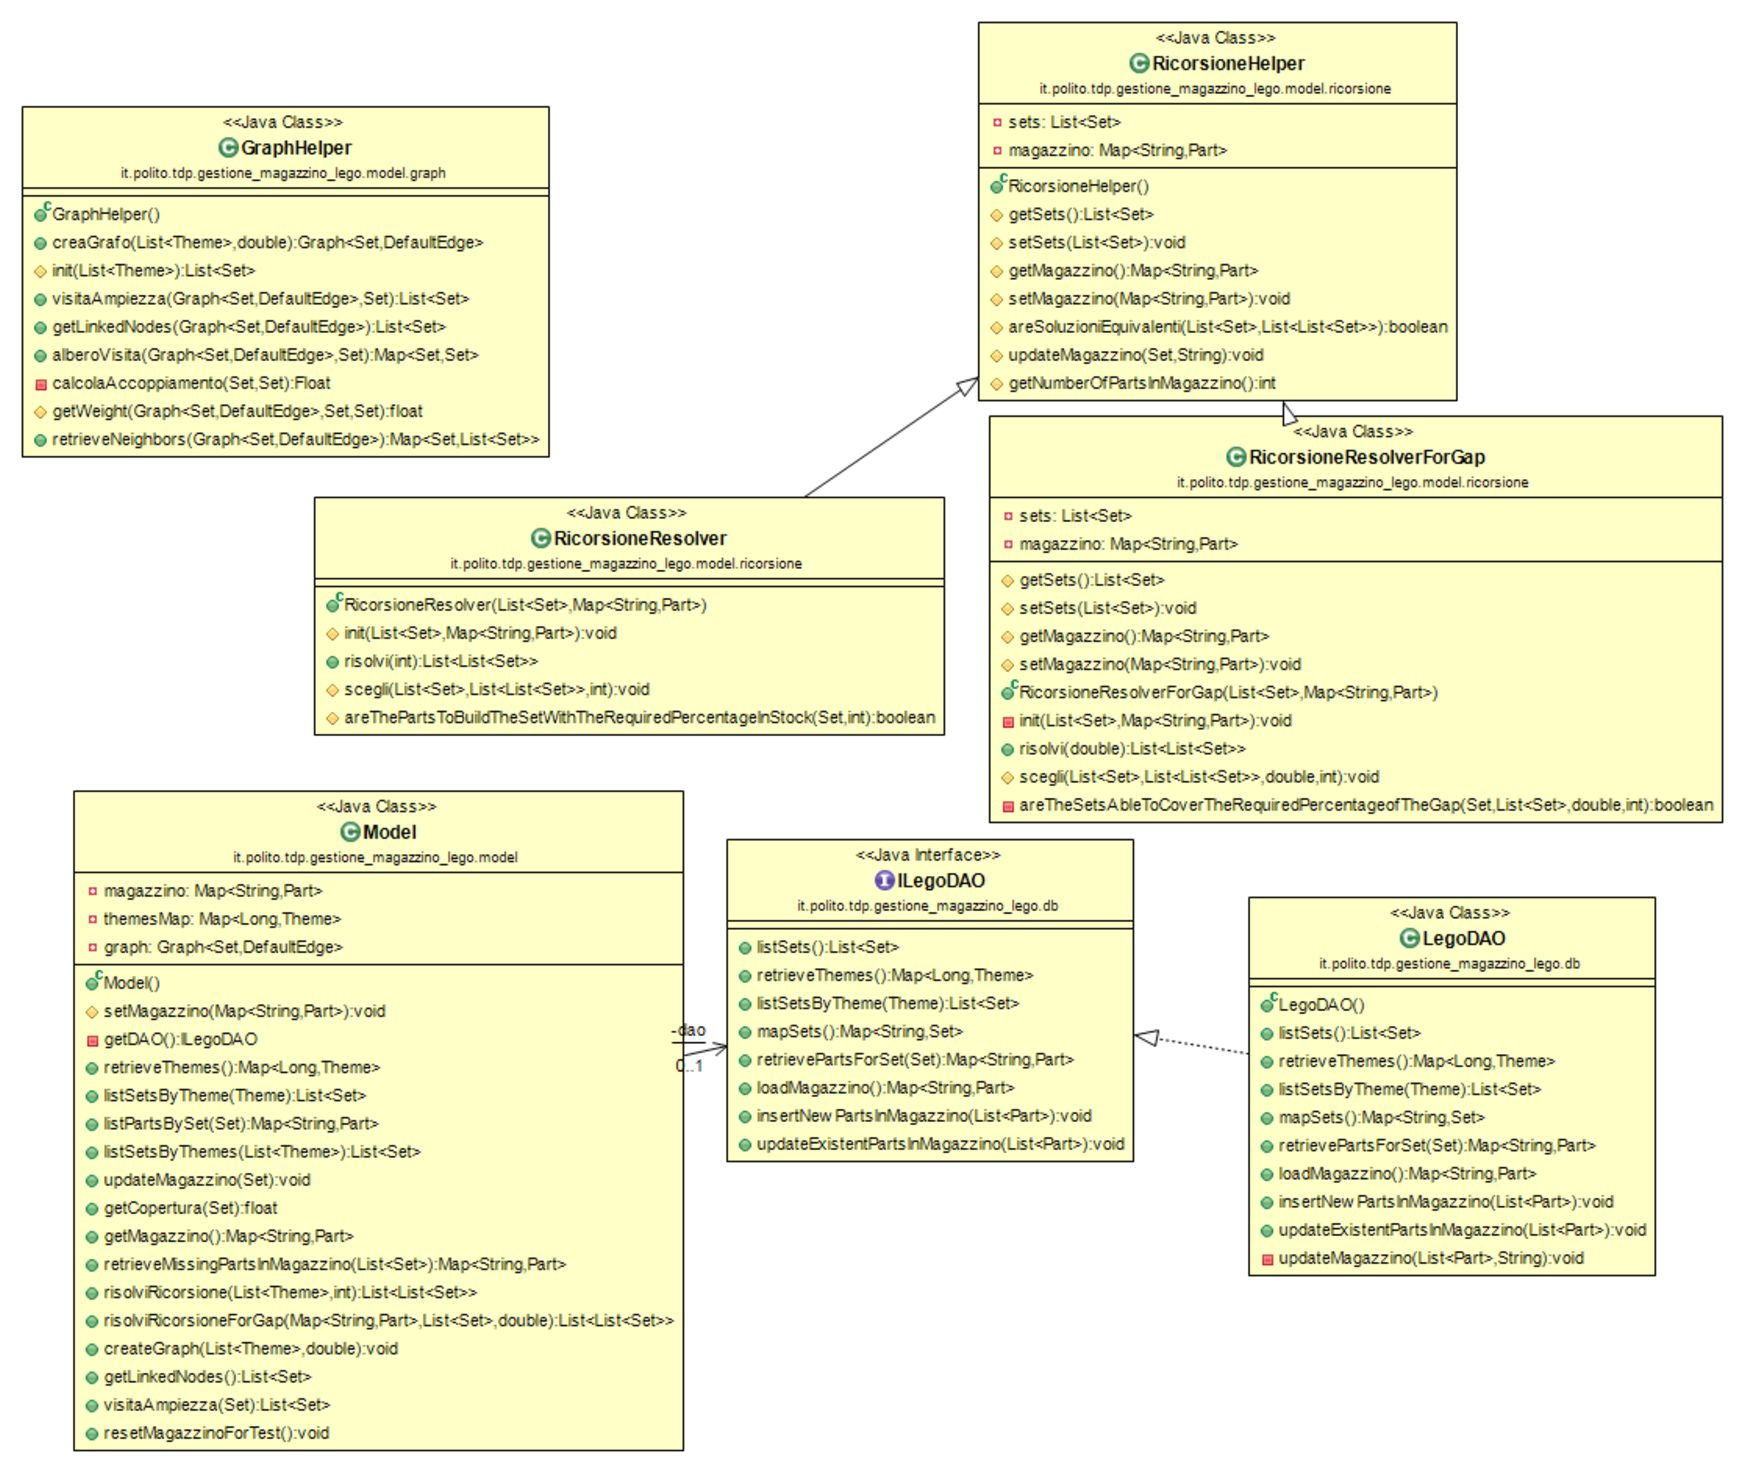
\includegraphics[scale=0.55]{diagramma_classi/uml_lego.eps}
\end{figure}




\chapter*{Interfaccia grafica}
\addcontentsline{toc}{chapter}{Interfaccia grafica}
L'interfaccia utente proposta presenta tre pannelli:
\begin{itemize}
\item la prima maschera offre semplici funzionalit� per riempire il magazzino simulando l'acquisto di un set. E' prevista la possibilit� di acquistare un set gi� esistente o uno nuovo con pezzi gi� presenti in magazzino. In questo caso si devono aggiornare le quantit� in magazzino con delle \texttt{UPDATE} e non delle \texttt{INSERT}. E' possibile anche visualizzare un semplice grafico a torta per avere un'indicazione di quanti pezzi ci sono in magazzino per costruire un determinato set
\item il secondo pannello offre la possibilit� di scegliere alcuni set e capire quali di questi possono essere costruiti con i pezzi in magazzino. Si ipotizza anche che l'utente possa decidere di accontentarsi di costruire parzialmente i set perch� poi acquister� i pezzi mancati singolarmente. Quindi � possibile impostare una percentuale di completamento.
\item l'ultima maschera infine dovr� elencare i pezzi mancanti  in magazzino per costruire totalmente o in parte un insieme di set e se interessa, cosa conviene acquistare per coprire le mancanze del magazzino.
\end{itemize}

\newpage

\section {Gestione magazzino}

\subsection {Caricamento di un set in magazzino}

\begin{figure}[htbp]
\centering
    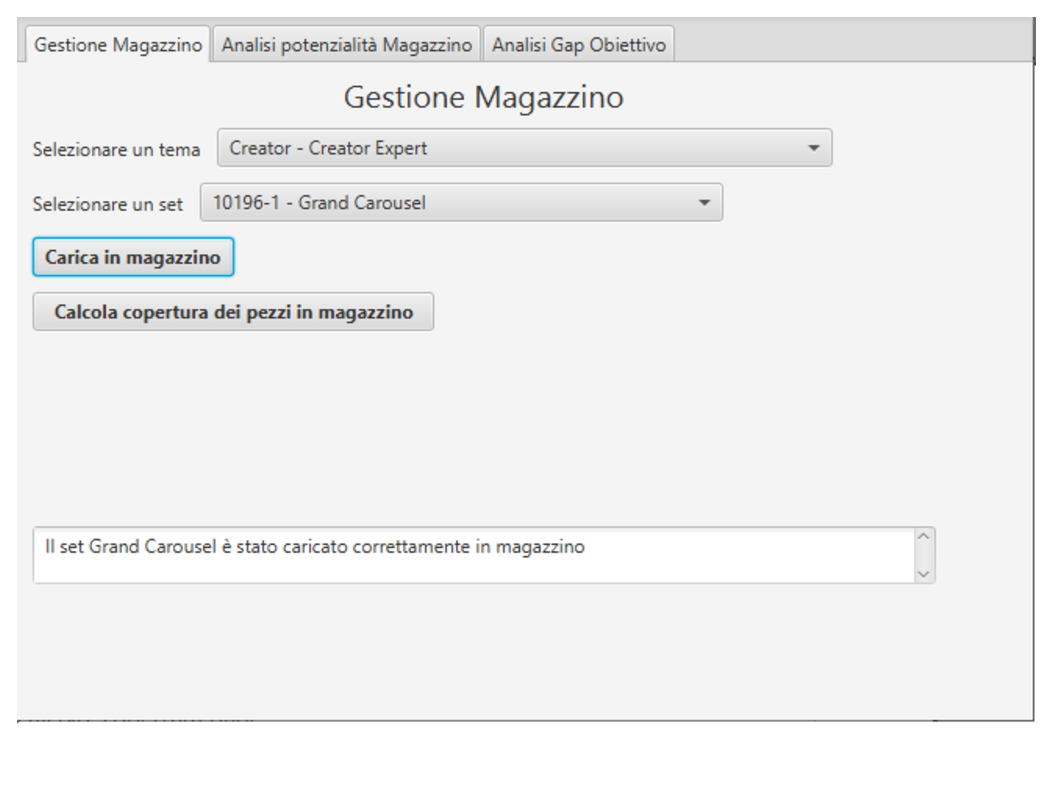
\includegraphics[scale=0.6]{interfaccia_grafica/caricamento_set_magazzino.eps}
\end{figure}


\subsection {Indicazione di quanto manca in magazzino per costruire un set}

\begin{figure}[htbp]
\centering
    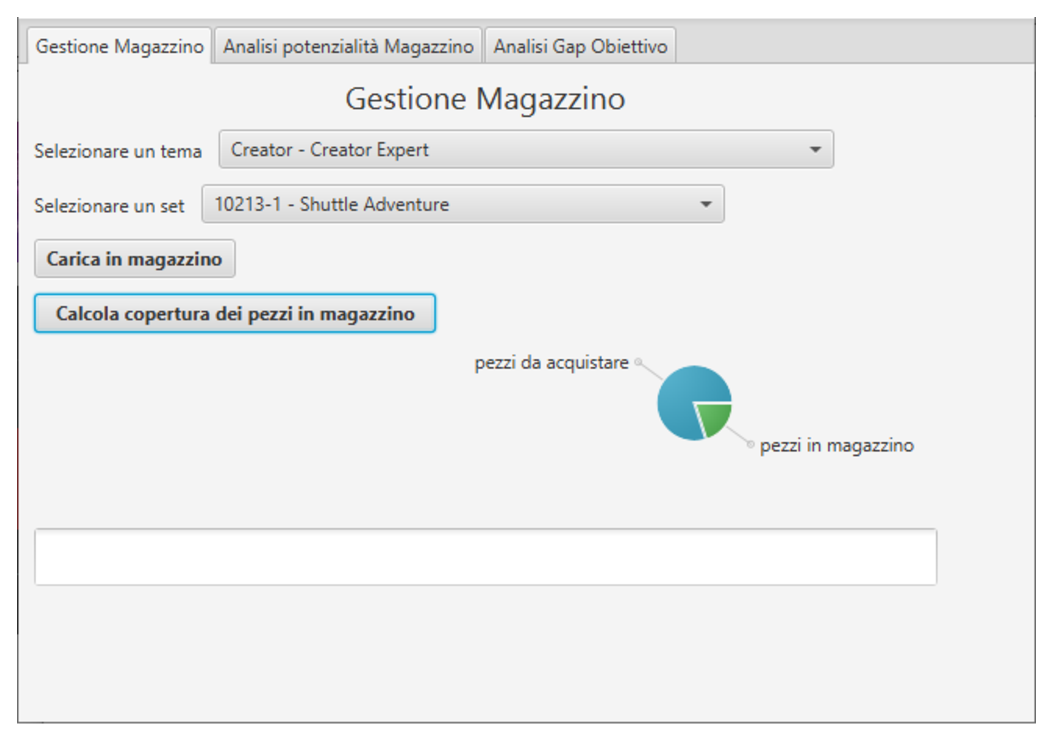
\includegraphics[scale=0.6]{interfaccia_grafica/calcolo_copertura.eps}
\end{figure}

\newpage


\section {Analisi potenzialit� del magazzino}

\begin{figure}[htbp]
\centering
    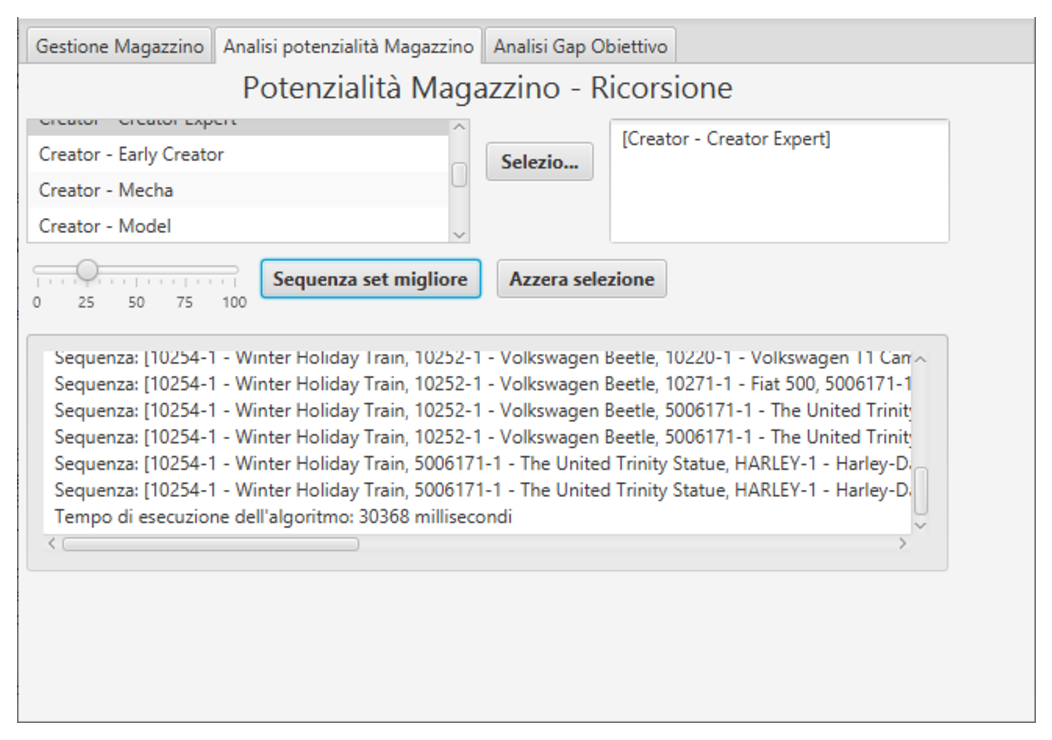
\includegraphics[scale=0.6]{interfaccia_grafica/ricorsione.eps}
\end{figure}

\section {Valutazioni per acquisti futuri}

\subsection {Creazione grafo e albero con set di interesse}

\begin{figure}[htbp]
\centering
    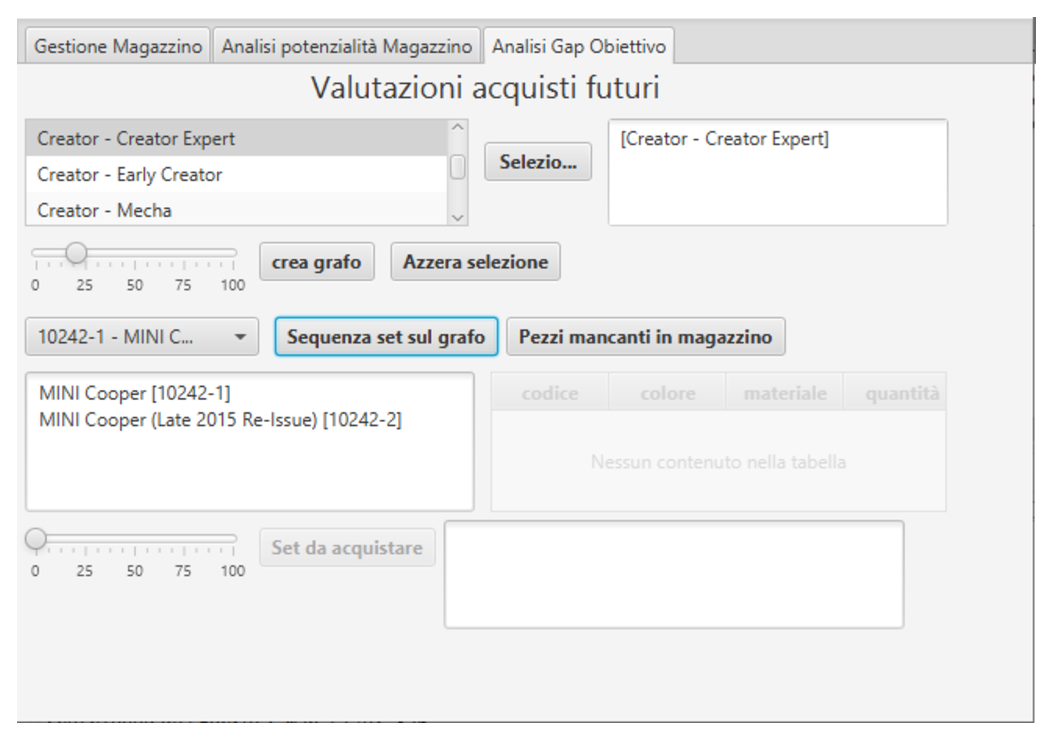
\includegraphics[scale=0.6]{interfaccia_grafica/creazione_grafo.eps}
\end{figure}

\newpage


\subsection {Pezzi mancanti in magazzino}

\begin{figure}[htbp]
\centering
    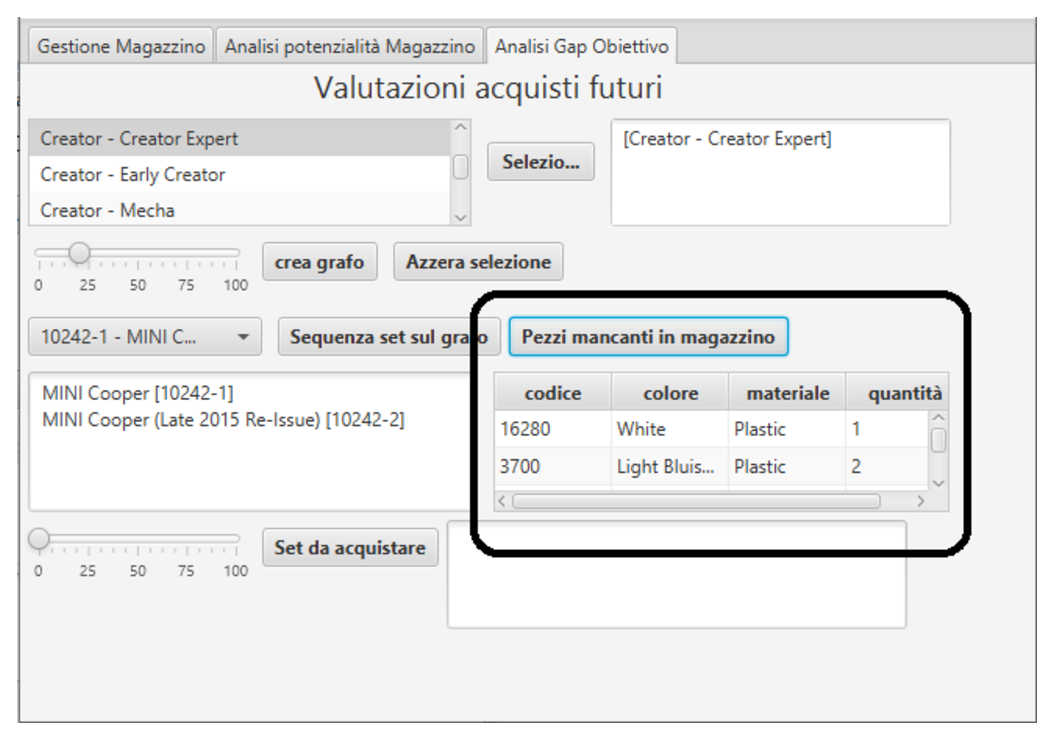
\includegraphics[scale=0.6]{interfaccia_grafica/parti_mancanti.eps}
\end{figure}

\subsection {Cosa conviene acquistare}

\begin{figure}[htbp]
\centering
    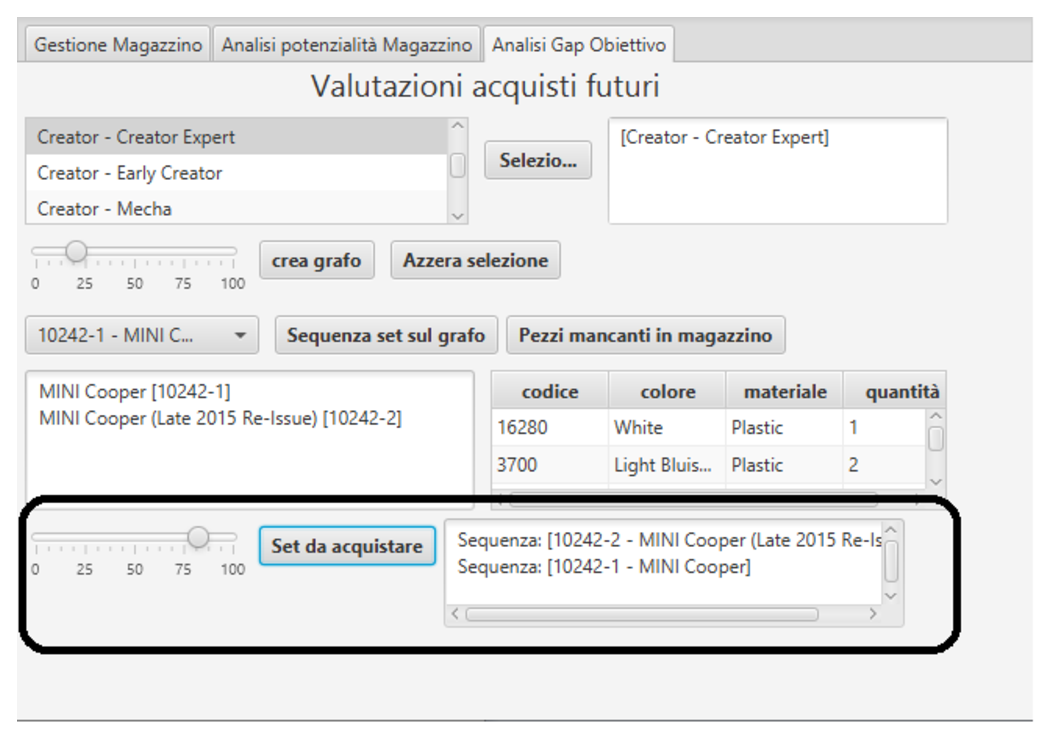
\includegraphics[scale=0.6]{interfaccia_grafica/gap.eps}
\end{figure}

\section {Video dimostrativo del software}

\url{https://youtu.be/JzkvN3o1dbM}

\chapter*{Risultati sperimentali}
\addcontentsline{toc}{chapter}{Risultati sperimentali}

Sia per l'analisi delle potenzialit� del magazzino sia per la ricerca dell'insieme di set pi� conveniente per colmare il gap per raggiungere un determinato obiettivo, si utilizza l'algoritmo della ricorsione. Si � quindi ritenuto utile valutare i tempi di esecuzione per un caso di studio semplice, ma indicativo della crescita esponenziale della complessit� del problema.

\section{Caso di studio}

Si suppone di partire da un magazzino vuoto e acquistare i seguenti tre set della serie Creator Export:
\begin{itemize}
\item Fiat 500 (10271-1)
\item London Bus (10258-1)
\item NASA Apollo 11 (10266-1)
\end{itemize}
Dopodich� si calcolano le sequenze di set che si possono costruire cambiando la percentuale di completamento a ogni prova. Si ottengono i risultati di seguito riportati nella tabella \ref{TAB:tempi_ricorsione} e nel grafico \ref{FIG:tempi_ricorsione}.
Si osserva come nel momento in cui la percentuale di completamento dei set scende sotto un valore sufficientemente basso a seconda della disponibilit� di pezzi in magazzino, i tempi aumentano in quanto il numero di soluzioni parziali valide aumenta considerevolmente.

\newpage

\vspace{0.5cm}
\begin{table}[htbp]
\begin{center}
\begin{tabular}{||c|c||}
\hline
{\bfseries percentuale di completamento dei set} & {\bfseries tempi in secondi}\\
\hline
\hline
90\% & 0.15\\
80\% & 0.15\\
70\% & 0.15\\
60\% & 0.15\\
50\% & 0.15\\
25\% & 30\\
20\% & 20\\
\hline
\hline
\hline
\end{tabular}
\caption {\label{TAB:tempi_ricorsione}  Tempi di esecuzione dell'algoritmo di ricorsione per diverse percentuali di completamento dei set}
\end{center}
\end{table}
\vspace{0.5cm}


\begin{figure}[htbp]
    \centering
    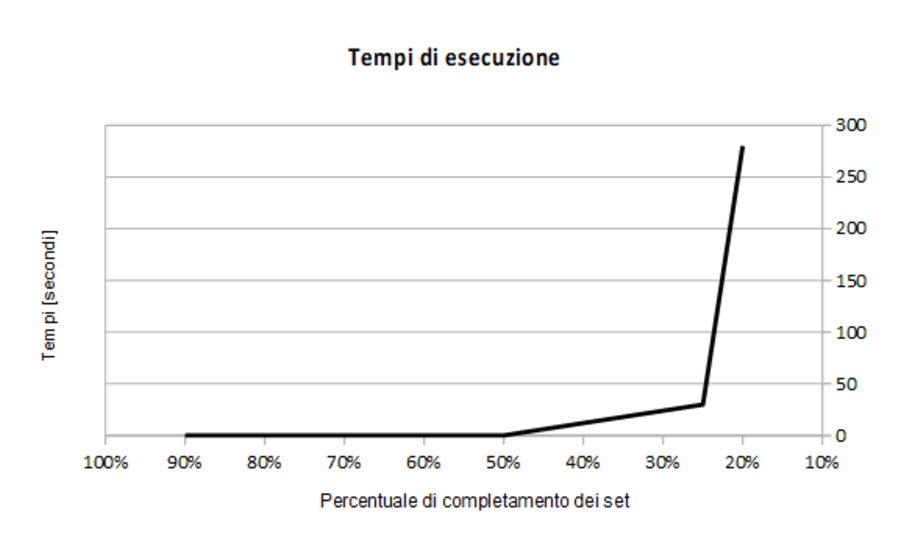
\includegraphics[scale=0.95]{risultati_sperimentali/tempi_ricorsione.eps}
\vspace{-5pt} \caption{Tempi dell'algoritmo di ricorsione}
\label{FIG:tempi_ricorsione}
\end{figure}
\vspace{0.5cm}



\chapter*{Conclusioni}
\addcontentsline{toc}{chapter}{Conclusioni}

La complessit� della base dati considerata in termini di numero di tabelle presenti e volume dei dati influisce molto sui tempi di esecuzione delle operazioni implementate.
Gli sviluppi sono stati quindi svolti utilizzando una classe DAO di test con pochi dati e semplici. Solo dopo aver verificato il corretto funzionamento degli algoritmi si � passati a lavorare sulla base dati vera.

Tra i punti di debolezza dell'applicazione si indica un'interfaccia grafica che deve essere migliorata dal punto di vista dell'usabilit�. Per esempio
\begin {itemize}
\item si dovrebbe poter scegliere un insieme di set non necessariamente collegati alla stessa serie;
\item manca la funzionalit� per poter aggiungere in magazzino pezzi acquistati singolarmente.
\end {itemize}

Senz'altro alcune parti del codice possono essere migliorate e ottimizzate. In molti punti si devono confrontare tra loro collezioni di oggetti con dimensioni non trascurabili. Un refactoring potrebbe influire sui tempi di esecuzione.

Alcuni risultati non totalmente corretti derivano da 
\begin {itemize}
	\item aver considerato solo i pezzi necessari per la costruzione del set e non anche quelli di riserva (attributo \texttt{is\_spare} della tabella \texttt{inventory\_parts})
\item non aver tenuto conto delle minifigure (tabelle \texttt{minifigs} e \\ \texttt{inventory\_minifigs})
\item in alcuni casi il numero di pezzi dichiarato nella tabella dei set (attributo \texttt{num\_parts}) non sempre corrisponde ai pezzi collegati al set nella tabella \texttt{inventory\_parts}. Quindi si � preferito calcolarlo ogni volta piuttosto che affidarsi a questa informazione
\end {itemize}

Infine un punto importante che potrebbe rappresentare un'importante miglioramento delle indicazioni ottenute dall'applicazione consiste nel assegnare un valore/peso a ogni pezzo. La base dati non fornisce informazioni a riguardo e quindi un semplice mattoncino 1x1 ha il valore di una ruota o di un motorino per un modello di veicolo. 
Se ci fossero queste informazioni, non sarebbero necessari molti interventi sul codice in quanto gi� ora per esempio la ricorsione � adatta a risolvere il problema dello zaino (rappresentato o dal magazzino oppure dal gap di pezzi che si vuole colmare).



\vfill
\begin{center}

\includegraphics{logo/licenza.eps}
\end{center}
\tiny{Quest'opera è distribuita con Licenza \url{http://creativecommons.org/licenses/by-nc-sa/2.5/it/} Creative Commons Attribuzione - Non commerciale - Condividi allo stesso modo 2.5 Italia}



\end{document}
